\section{Theoretical Analysis}
\label{sec:analysis}

We analyse the circuit shown in Figure~\ref{fig:rc} for t<0 using the nodal method.
The nodes are numbered according to what's shown in the picture.
In this first instance we are working in a steady state, where no current is flowing through the capacitor: we can replace it with an open circuit.
After doing this, it is clear that all the components we are working with are linear and so we will need to solve a system of linear equations to determine the initial values for the subsequent analysis.
This way, we’ve ran the nodal method and solved the linear system on GNU Octave.
\subsection{Node Analysis for t<0}
Knowing that V4=0 since it is connected to the ground:
\begin{equation}
\begin{pmatrix}
1 & 0 & 0 & 0 & 0 & 0 & 0\\
-G1 & G1+G2+G3 & -G2 & -G3 & 0 & 0 & 0\\
0 & Kb+G2 & -G2 & -Kb & 0 & 0 & 0\\
-G1 & G1 & 0 & G4 & 0 & G6 & 0\\
0 & 0 & 0 & 0 & 0 & -G6-G7 & G7\\
0 & 0 & 0 & 1 & 0 & G6*Kd & -1\\
0 & -G3 & 0 & G3+G4+G5 & -G5 & G6 & 0
\end{pmatrix}
\begin{pmatrix}
V1\\
V2\\
V3\\
V5\\
V6\\
V7\\
V8
\end{pmatrix}
=
\begin{pmatrix}
Vs\\
0\\
0\\
0\\
0\\
0\\
0
\end{pmatrix}
\end{equation}
We can also easily obtain the current values in the various branches through Ohm's law. This yields the following results:
\begin{table}[h]
  \centering
  \begin{tabular}{|l|r|}
    \hline    
    {\bf Name} & {\bf Value [mA and V]} \\ \hline
    @$I_{R1}$ & 0.219167 \\ \hline 
@$I_{R2}$ & 0.229771 \\ \hline 
@$I_{R3}$ & 0.010604 \\ \hline 
@$I_{R4}$ & 1.185502 \\ \hline 
@$I_{R5}$ & 0.229771 \\ \hline 
@$I_{R6}$ & 0.966335 \\ \hline 
@$I_{R7}$ & 0.966335 \\ \hline 
@$I_{b}$ & -0.229771 \\ \hline 
@$I_{C}$ & 0.000000 \\ \hline 
@$I_{Vs}$ & 0.219167 \\ \hline 
@$I_{Kd}$ & 0.966335 \\ \hline 
$V_{1}$ & 5.113399 \\ \hline 
$V_{2}$ & 4.889447 \\ \hline 
$V_{3}$ & 4.428712 \\ \hline 
$V_{4}$ & 0.000000 \\ \hline 
$V_{5}$ & 4.921444 \\ \hline 
$V_{6}$ & 5.620907 \\ \hline 
$V_{7}$ & -1.953900 \\ \hline 
$V_{8}$ & -2.927814 \\ \hline 
 
  \end{tabular}
  \caption{Theoretical analysis results for time, t, inferior to 0 . (A variable preceded by @ is of type {\em current})}
  \label{tab:nodal}
\end{table}

\subsection{Equivalent Resistor}
In order to compute the equivalent resistor we ran a nodal analysis, making Vs=0 and replacing the capacitor with a voltage source Vx=V6-V8 as calculated in the previous step. This is made to ensure that the voltage in the capacitor is continuous since it does so in reality: this is a capacitor discharging through a resistance, any discontinuity in voltage would require an infinite amount of current. 
\begin{equation}
\begin{pmatrix}
1 & 0 & 0 & 0 & 0 & 0 & 0\\
-G1 & G1+G2+G3 & -G2 & -G3 & 0 & 0 & 0\\
0 & Kb+G2 & -G2 & -Kb & 0 & 0 & 0\\
-G1 & G1 & 0 & G4 & 0 & G6 & 0\\
0 & 0 & 0 & 0 & 0 & -G6-G7 & G7\\
0 & 0 & 0 & 1 & 0 & G6*Kd & -1\\
0 & 0 & 0 & 0 & 1 & 0 & -1
\end{pmatrix}
\begin{pmatrix}
V1\\
V2\\
V3\\
V5\\
V6\\
V7\\
V8
\end{pmatrix}
=
\begin{pmatrix}
0\\
0\\
0\\
0\\
0\\
0\\
Vx
\end{pmatrix}
\end{equation}

With the following definitions:
\begin{equation}
V_x=V_6-V_8;
\end{equation}
\begin{equation}
I_x=\frac {V_6-V_5}{R_5}+\frac {V_3-V_2}{R_2};
\end{equation}
\begin{equation}
Req=\frac {V_x}{I_x}
\end{equation}
We were able to obtain the following values, laying the foundation for the natural solution:
\begin{table}[h]
  \centering
  \begin{tabular}{|l|r|}
    \hline    
    {\bf Name} & {\bf Value} \\ \hline
    $V_{x}$ & 8.548721 V\\ \hline
@$I_{x}$ & 2.808224 mA\\ \hline
$R_{eq}$ & 3.044174 kOhm\\ \hline
$tau$ & 3.059522 ms\\ \hline 
  \end{tabular}
  \caption{Theoretical analysis calculations for $R_{eq}$ and $tau$.}
  \label{tab:equivalent}
\end{table}
\subsection{Natural solution}
The general solution for RC circuits, making use of the computations in the previous section, yields:
\begin{equation}
V_{6n}(t)=V_xexp(-\frac{t}{RC});
\end{equation}
From this equation, we obtained the following plot, which depicts the first twenty milisseconds of the circuit's natural response.
\begin{figure}[h] \centering
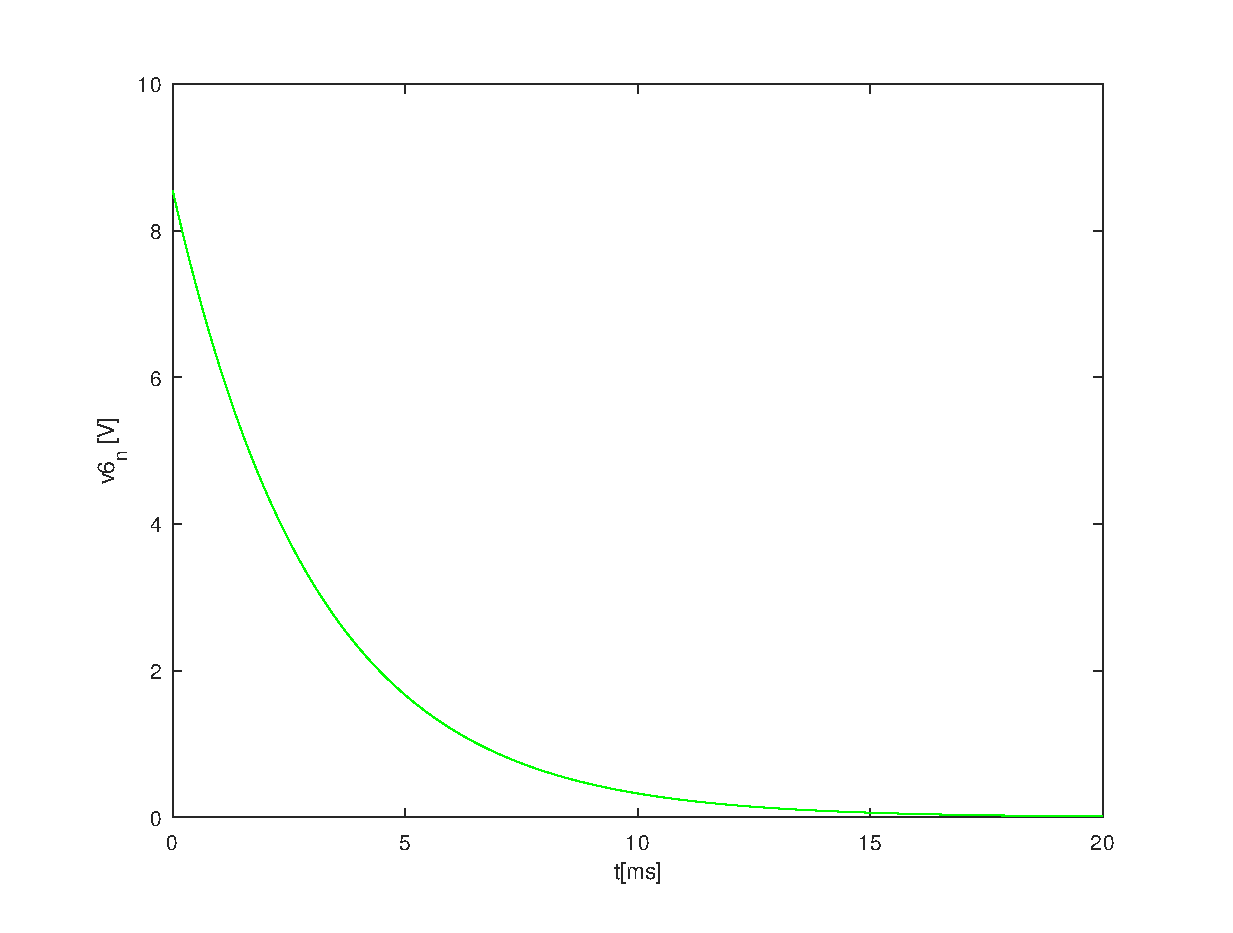
\includegraphics[width=0.8\linewidth]{natural.eps}
\caption{Natural solution to $V_{6}$ node voltage.}
\label{fig:current}
\end{figure}

\subsection{Forced and final total solution}
In order to study the forced response of the system, we performed a nodal analysis to obtain the phasor voltage in every node by solving the following system:
\begin{equation}
\begin{pmatrix}
1 & 0 & 0 & 0 & 0 & 0 & 0\\
-G1 & G1+G2+G3 & -G2 & -G3 & 0 & 0 & 0\\
0 & Kb+G2 & -G2 & -Kb & 0 & 0 & 0\\
-G1 & G1 & 0 & G4 & 0 & G6 & 0\\
0 & 0 & 0 & 0 & 0 & -G6-G7 & G7\\
0 & 0 & 0 & 1 & 0 & G6*Kd & -1\\
0 & -G3 & 0 & G3+G4+G5 & -G5-jwC & G6 & jwC
\end{pmatrix}
\begin{pmatrix}
V1\\
V2\\
V3\\
V5\\
V6\\
V7\\
V8
\end{pmatrix}
=
\begin{pmatrix}
-j\\
0\\
0\\
0\\
0\\
0\\
0
\end{pmatrix}
\end{equation}
We then get these values:
\begin{table}[h]
  \centering
  \begin{tabular}{|l|r|}
    \hline    
    {\bf Name} & {\bf Value [V]} \\ \hline
    V1 & 0.000000-1.000000j\\ \hline
V2 & 0.000000-0.956203j\\ \hline
V3 & 0.000000-0.866099j\\ \hline
V5 & 0.000000-0.962460j\\ \hline
V6 & -0.086733+0.568065j\\ \hline
V7 & -0.000000+0.382114j\\ \hline
V8 & 0.000000+0.572577j\\ \hline 
  \end{tabular}
  \caption{Phasor voltage in every node.}
  \label{tab:phasor}
\end{table} \par
We're now able to make sense of the equation that describes the forced solution to the voltage at node 6.
\begin{equation}
V_{6f}(t)=V_{6r}cos(wt+V_{6\phi})=-0.086733cos(2000\pi*t+1.7223);
\end{equation}
\subsection{Final total solution}
Now we convert the phasors to real time functions and consider an angular frequency of $2000\pi$. By superimposing both natural and forced responses we get the total solution:
\begin{equation}
V_{6}(t)=V_{6f}(t)+V_{6n}(t);
\end{equation}
By plotting both $V_s(t)$ and $V_6(t)$ from -5ms to 20ms we can see that both plots are constant before t=0. The evolution of V6 is as expected, as we can clearly see the negative exponential behaviour as well as the induced frequency.
\begin{figure}[h] \centering
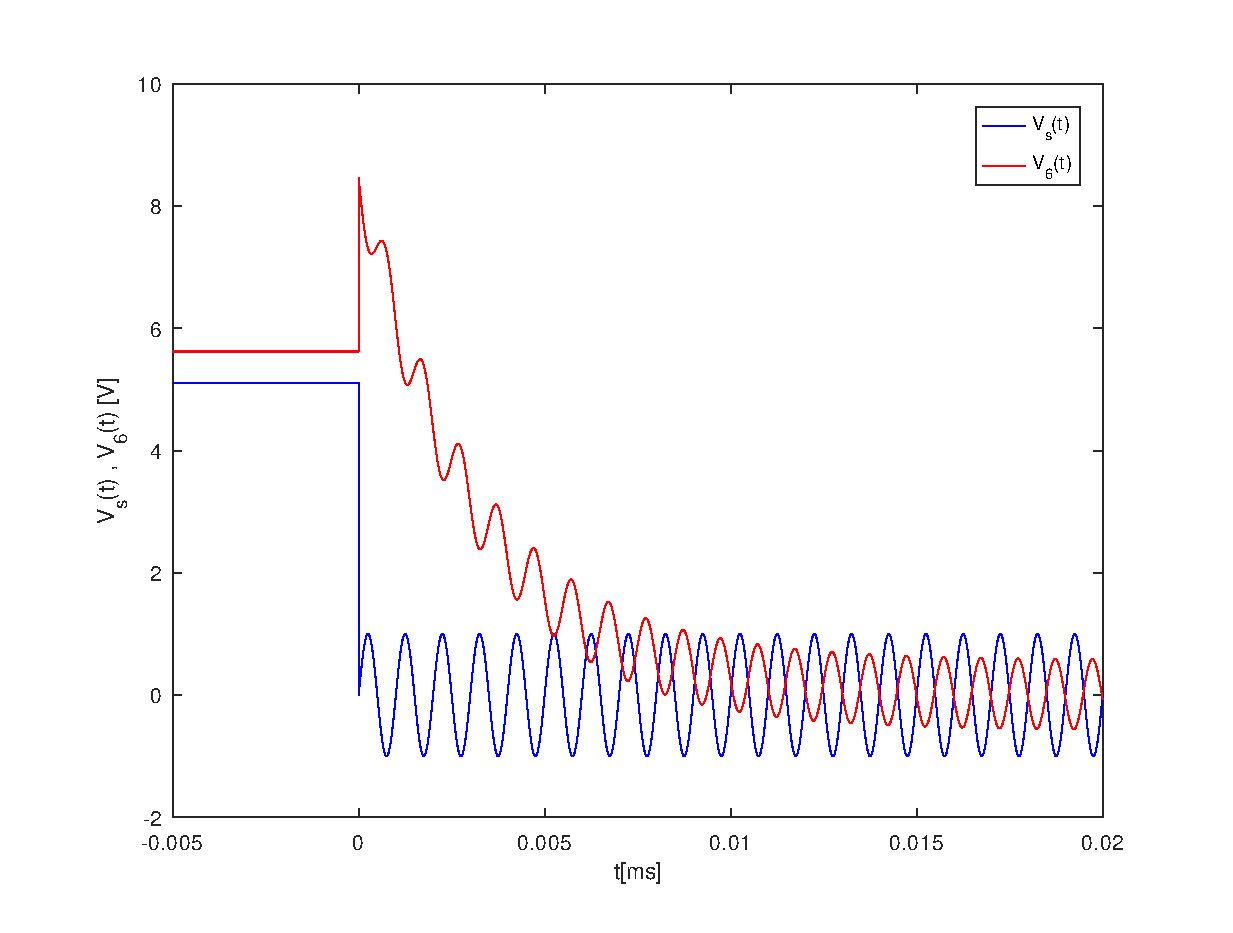
\includegraphics[width=0.7\linewidth]{total.eps}
\caption{Total solution to $V_{6}$ node voltage.}
\end{figure}\pagebreak

\subsection{Frequency response}

\begin{figure}[h] 
	\centering
\begin{minipage}[b]{0.45\linewidth}	
	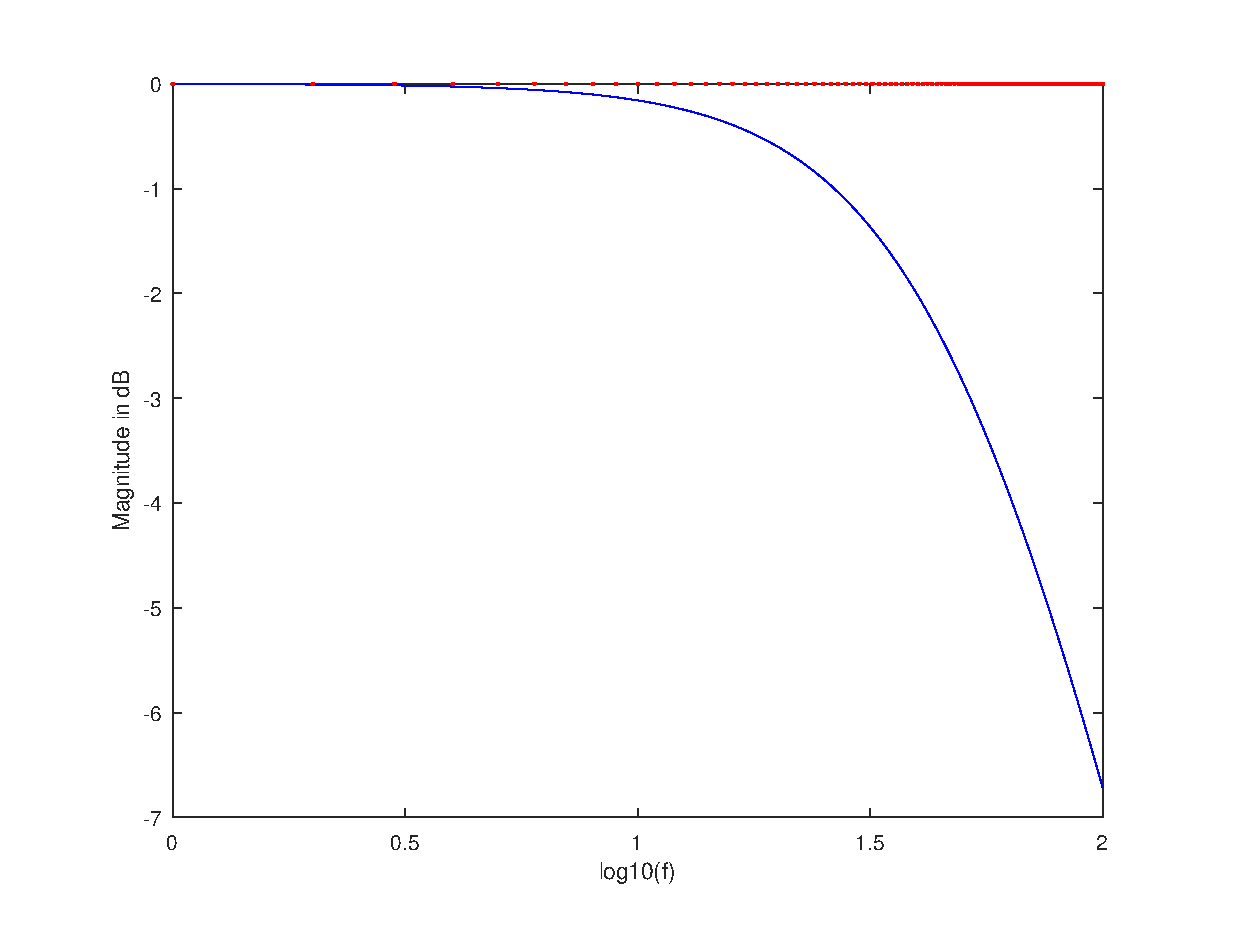
\includegraphics[width=\linewidth]{magnitude.eps}
\caption{Total solution to $V_{6}$ node voltage.}
\end{minipage}
\hfill
\begin{minipage}[b]{0.45\linewidth}
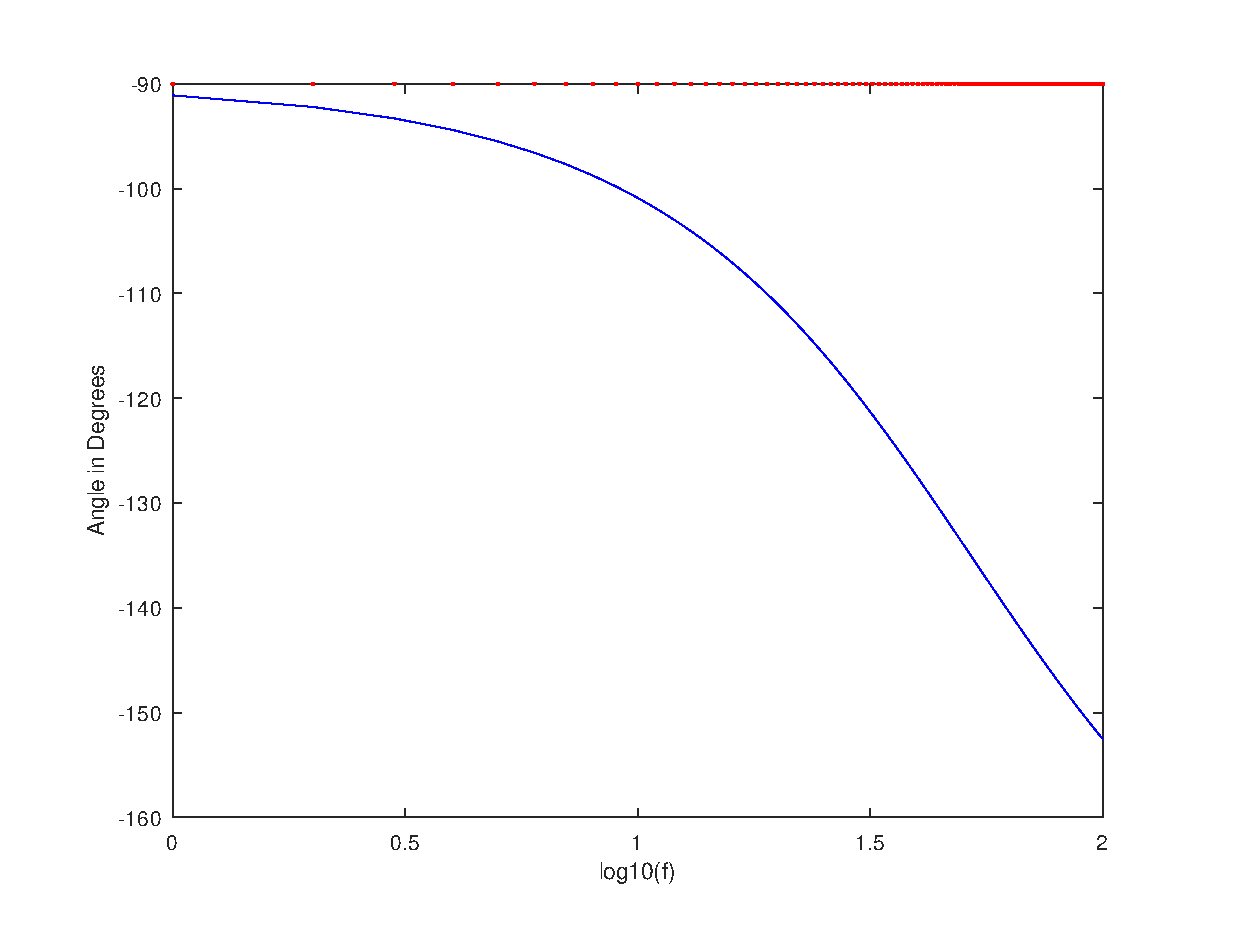
\includegraphics[width=\linewidth]{angle.eps}
\caption{Total solution to $V_{6}$ node voltage.}
\end{minipage}
\end{figure}
